% Technical appendix. The main file supplies the Beamer preamble,
% \source{...}, and \takeaway{...}. Counts below are applicant-years or
% simulated pupil--draw events as indicated; no new experiment is reported.

\begin{frame}{Outcomes and denominators}
\small
For menu policy $D$, let $M_D(i)$ be the replayed assignment and $\ell_i$
the pupil's historical April enrollment school.
\[
 H(D)=\sum_{i\in L}\mathbf{1}\{\exists j\in D_i:\operatorname{school}(j)=\ell_i\},
 \qquad
 P_L(D)=\sum_{i\in L}\mathbf{1}\{M_D(i)\ne\bot\}.
\]
\begin{itemize}
  \item $L$: 1,969,120 linked applicant-years in 2022--25.
  Full initial-offer reconstruction: 2,044,649 applicant-years.
  \item Chile differences use the same linked denominator:
  $100\,\Delta H/|L|=+0.236$ pp and
  $100\,\Delta P_L/|L|=-0.0848$ pp.
  \item NYC coverage is conditional on a full-information match;
  NYC placement includes everyone in the sampled market.
\end{itemize}
\takeaway{A historical-school hit is neither an assignment nor a welfare measure.}
\source{\texttt{findings/chile/cohort\_comparison.csv}; \texttt{findings/README.md}.}
\end{frame}

\begin{frame}{The Chile result depends on the comparator}
\small
Rank-informed menus minus each baseline, on the same linked sample:
\begin{center}
\begin{tabular}{lrr}
\hline
Baseline & April-school hits & Placements\\
\hline
Rank-blind & $+4,638$ & $-1,670$\\
Family's first five discretionary courses & $+9,800$ & $+8,143$\\
\hline
\end{tabular}
\end{center}
\begin{itemize}
  \item The rank-blind comparison has 2,397 gross exits and 727 entrants.
  Full-population net placement changes by $-1,834$; the linked change is $-1,670$.
  \item The 145,450 linked pupils with no historical initial offer lose
  1,270 places against rank-blind and 2,860 against first-five.
  \item This group is 7.39\% of the linked sample and bears 76.05\%
  of the net decline against rank-blind.
\end{itemize}
\takeaway{A better aggregate comparator does not remove the access problem.}
\source{\texttt{findings/chile/cohort\_comparison.csv}; \texttt{group\_comparison.csv}; \texttt{all\_population\_spillovers.csv}.}
\end{frame}

\begin{frame}{The fixed-menu seat-retention problem}
\small
\setlength{\abovedisplayskip}{3pt}
\setlength{\belowdisplayskip}{3pt}
Let $A_i$ and $B_i$ be the rank-blind and rank-informed course menus.
Keep shared courses and the original quota:
\[
 \mathcal D=\{D: A_i\cap B_i\subseteq D_i\subseteq A_i\cup B_i,
                 \ |D_i|=|A_i|\ \text{for every }i\}.
\]
For a lottery draw $s$, define the baseline recipients and gross exits:
\[
 R_s=\{i:M_A^s(i)\ne\bot\},\qquad
 X_s(D)=\sum_{i\in R_s}\mathbf{1}\{M_D^s(i)=\bot\}.
\]
\[
 \max_{D\in\mathcal D}\ H(D)-H(A)
 \quad\text{subject to}\quad X_s(D)=0\quad\text{for every }s\in S.
\]
\begin{itemize}
  \item One menu policy per cohort must work across the entire draw panel $S$.
  Protection includes nonlinked pupils; $H$ scores only linked pupils.
  \item Old coverage hits may be lost. School and seat type may change.
  April labels make this optimization a hindsight benchmark.
\end{itemize}
\source{\texttt{findings/chile/README.md}, protection definition; pinned paper: \texttt{retention-evidence.tex}.}
\end{frame}

\begin{frame}{Stable witnesses under fixed priorities}
\small
\setlength{\abovedisplayskip}{3pt}
\setlength{\belowdisplayskip}{3pt}
$x_{ij}\in\{0,1\}$ selects a menu; $y^s_{ij}\in\{0,1\}$ is an assignment witness.
For every draw $s$:
\[
 y^s_{ij}\le x_{ij},\qquad
 \sum_j y^s_{ij}\le1,\qquad
 \sum_i y^s_{ij}\le q_j,\qquad
 \sum_j y^s_{ij}=1\quad(i\in R_s).
\]
For each candidate pair with $q_j>0$, rule out blocking:
\[
 q_j\sum_{k:\,k\succeq_i j}y^s_{ik}
 +\sum_{h:\,h\succ_j^s i}y^s_{hj}
 \ \ge\ q_j x_{ij}.
\]
\begin{itemize}
  \item Displayed $j$: either $i$ gets a weakly better course,
  or $j$ fills with higher-priority pupils.
  \item Applicant optimality: a retaining stable witness exists iff
  applicant-proposing DA retains everyone in $R_s$.
\end{itemize}
\takeaway{Fixed strict responsive priorities are essential;
sibling rules need separate treatment.}
\source{\texttt{findings/chile/README.md}, linked pinned proof: \texttt{retention-theory.tex}.}
\end{frame}

\begin{frame}{Hardness: competing edits}
\small
\setlength{\parskip}{0pt}
Four pupils per graph vertex; unit seats; only $z$ is shared.
\begin{center}
\begin{tabular}{cll}
\hline
Pupil & Full preference list & Permitted menu\\
\hline
$t_i$ & $p_i,x_i,b_i$ & $(p_i,b_i)$ or $(p_i,x_i)$\\
$g_i$ & $p_i,q_i$ & fixed full list\\
$h_i$ & $x_i,z,r_i$ & fixed full list\\
$d_i$ & $r_i,s_i$ & fixed full list\\
\hline
\end{tabular}
\end{center}
Selecting vertex $i$ changes $t_i$'s menu from $(p_i,b_i)$ to $(p_i,x_i)$.
\begin{itemize}
  \item Edge draw $\{u,v\}$: common priority puts $d$ pupils first,
  then $(g_i,t_i)$ at endpoints and $(t_i,g_i)$ elsewhere; $h$ pupils last.
  \item Selected endpoint: $g_i$ takes $p_i$, $t_i$ takes $x_i$.
  Displaced $h_i$ needs $z$ because $d_i$ holds $r_i$.
\end{itemize}
\takeaway{Both endpoints selected $\Rightarrow$ two displaced pupils need the one seat at $z$.}
\source{\texttt{findings/chile/README.md}, linked pinned proof: \texttt{retention-theory.tex}.}
\end{frame}

\begin{frame}{Hardness: correctness of the reduction}
\small
Reference draw: priority groups $g,t,h,d$, highest first.
\begin{itemize}
  \item Full-list DA gives $t_i$ its target $x_i$.
  All other targets lie on fixed menus: one hit per selected vertex.
  \item Reference draw always retains everyone: displaced $h_i$ has $r_i$;
  displaced $d_i$ has $s_i$.
  \item Edge draw retains everyone iff its endpoints are not both selected.
  Old menus always retain everyone.
\end{itemize}
\[
 \text{retaining menu with gain at least }K
 \quad\Longleftrightarrow\quad
 \text{independent set of size at least }K.
\]
DA checks the explicit panel in polynomial time.
\takeaway{NP-complete with unit seats, common priorities per draw,
and menus of length at most three.}
\source{\texttt{findings/chile/README.md}, linked pinned proof: \texttt{retention-theory.tex}.}
\end{frame}

\begin{frame}{Bounding the hindsight optimum}
\small
Same menu family; 1,024 design draws per cohort, 2022--24.
\begin{center}
\begin{tabular}{lrrr}
\hline
 & 2022 & 2023 & 2024\\
\hline
Exact course and seat type: optimum & 96 & 111 & 107\\
Seat retention: attained & 170 & 199 & 273\\
Seat retention: upper bound & 1,350 & 1,564 & 1,706\\
\hline
\end{tabular}
\end{center}
\begin{itemize}
  \item \textbf{Lower:} add missed April schools; withdraw swaps implicated
  in exits; re-clear all national draws. Gain 642 hits; lose no old hit;
  zero exits.
  \item \textbf{Upper:} intersect row restrictions from priority cutoffs,
  capacity paths and unavoidable displacement.
  Of 4,823 possible new hits, 4,620 survive.
\end{itemize}
\takeaway{Surviving upper-bound gains need not coexist. This is an optimization
gap on a finite panel, not a confidence interval.}
\source{\texttt{findings/chile/retention\_bounds.csv}; pinned paper: \texttt{retention-evidence.tex}.}
\end{frame}

\begin{frame}{The remaining retention interval}
\small
Additional historical-school hits, summed over 2022--24.
\begin{center}
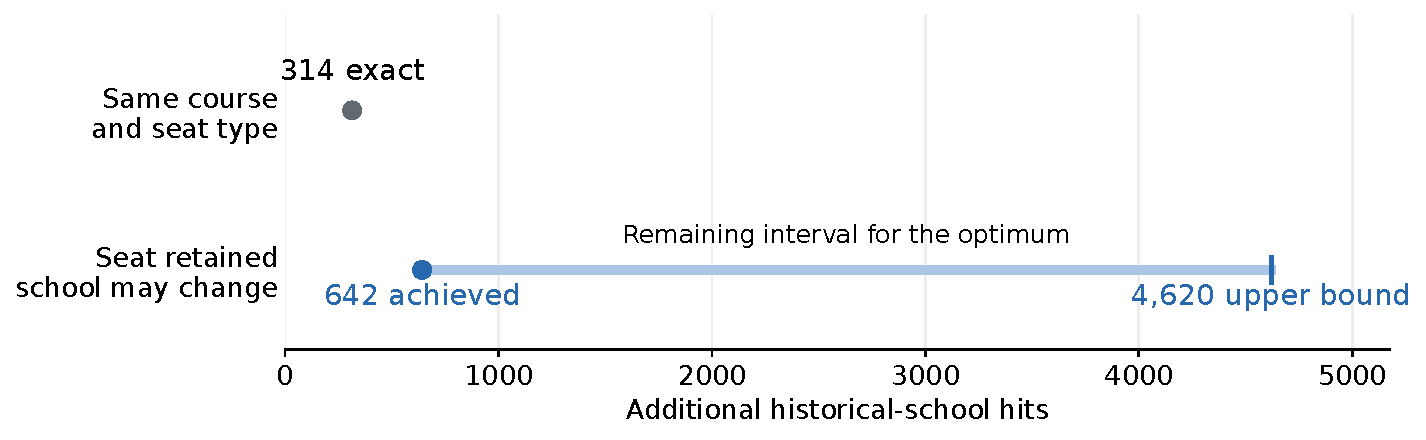
\includegraphics[width=.93\textwidth]{figures/retention.pdf}
\end{center}
The 642-hit construction exceeds the 314-hit exact-assignment ceiling.
The 4,620 upper bound leaves the optimum unresolved.
\source{Fixed common/union menus, 1,024 design lotteries per cohort. Hindsight optimization bounds, not confidence intervals or prospective policy gains. Source: \texttt{findings/chile/retention\_bounds.csv}.}
\end{frame}

\begin{frame}{Retention under every lottery order}
\small
\begin{enumerate}
  \item Certify a common option: continuity, ample total capacity,
  or more category seats than possible higher-priority rivals.
  \item Close pupils lacking guarantees under active competitors at scarce
  courses and relevant older relatives. Freeze active memberships there.
  \item Fill remaining slots by submitted rank; keep common courses and quotas.
\end{enumerate}
\medskip
\textbf{Proof idea.} Outside the closure, guarantees remain.
Inside, relevant interactions stay fixed. Induct over grades and proposals.
\takeaway{All strict ordinary orders are covered, holding reports,
capacities, family links and special rankings fixed.}
\source{\texttt{findings/chile/README.md}; pinned paper: \texttt{retention-evidence.tex}, \texttt{retention/structural/structural.cpp}.}
\end{frame}

\begin{frame}{Learning before assignment}
\small
\begin{itemize}
  \item \textbf{Labels:} 2021 applicants' April 2022 enrollment.
  \item \textbf{Features:} submitted rank and frozen 2019 offer scores;
  175 probability cells with shrinkage.
  \item \textbf{Decision:} maximize predicted distinct-school coverage within
  design-draw restrictions. Keep common courses and quotas.
  \item \textbf{Holdout:} menus frozen before later-label scoring and fresh
  lottery draws; the 2022--24 populations are unchanged.
\end{itemize}
\begin{center}
\setlength{\tabcolsep}{10pt}
\begin{tabular}{lrrr}
\hline
Rule & New hits & Old hits lost & Net\\
\hline
Structural & 115 & 87 & $+28$\\
Learned & 134 & 84 & $+50$\\
\hline
\end{tabular}
\end{center}
\source{\texttt{findings/chile/prospective.csv}; pinned paper: \texttt{retention-evidence.tex}, \texttt{retention/policy/PLAN.md}.}
\end{frame}

\begin{frame}{Failures on fresh lotteries}
\small
Paired baselines; counts are simulated pupil--draw events.
\begin{center}
\begin{tabular}{llrrr}
\hline
Draw generator & Rule & Exits & Entrants & School switches\\
\hline
384 course draws & Structural & 0 & 0 & 9,643\\
 & Learned & 1 & 104 & 3,445\\
96 family-ticket draws & Structural & 0 & 0 & 2,417\\
 & Learned & 1 & 28 & 879\\
\hline
\end{tabular}
\end{center}
\begin{itemize}
  \item Course failure: 2023, draw 42. Family-ticket failure: 2022;
  two entrants and one exit produce a net gain of one place.
  \item Same applicant populations; pupils recur across draws.
  Neither rule changes coverage for 115,626 initially unoffered linked pupils.
\end{itemize}
\takeaway{A positive headcount change can still break an individual retention promise.}
\source{\texttt{findings/chile/prospective.csv}; \texttt{findings/chile/prospective\_draws.csv}.}
\end{frame}

\begin{frame}{Institutional and behavioral limits}
\small
\begin{itemize}
  \item \textbf{Fidelity:} every released course/no-offer outcome matches
  across 2,044,649 applicant-years, using grade order, family links and seat types.
  \item \textbf{Replay:} menus bind; reports and supply stay fixed.
  Historical fit cannot validate responses to advice.
  \item \textbf{2021 entry grades:} unchanged-menu pupils bear 237 of 309
  net placement losses. This is simulated interference.
  \item \textbf{Field trial:} public data lack treatment arms and personalized
  recommendations. Replay losses are not experimental effects.
\end{itemize}
\takeaway{Deployment claims require evidence about how families use advice.}
\source{\texttt{findings/chile/historical\_fidelity.csv}; \texttt{field\_cohort.csv}; pinned paper: \texttt{field-validation.tex}.}
\end{frame}

\begin{frame}{Reproduction and open questions}
\small
\textbf{Reproduce the released presentation evidence}
\begin{itemize}
  \item \texttt{python3 findings/chile/rebuild.py} verifies 35 source hashes
  and rebuilds eight summaries.
  \item Checks accounting, draw coverage and paired baselines;
  it does not rerun admissions from pupil records.
\end{itemize}
\medskip
\textbf{Questions the current results do not settle}
\begin{itemize}
  \item Close the 642--4,620 optimization gap.
  \item Improve excluded pupils' access while retaining every recipient.
  \item Test individual losses under NYC anchors and nonbinding advice.
\end{itemize}
\takeaway{Next: measure exits and rank changes under the NYC anchors.}
\source{\texttt{findings/chile/provenance.json}; \texttt{findings/chile/rebuild.py}; \texttt{findings/chile/README.md}.}
\end{frame}

\begin{frame}{Relation to coordinated recommendations}
\small
\textbf{Existing work.} Ashlagi, Braverman, Kanoria and Shi (2020) study
informative signals and match recommendations for clearing matching markets
efficiently. Coordination is an established research direction.
\par\medskip
\textbf{Our question.} On fixed reports, can one edited menu policy improve
historical-school coverage while retaining every baseline recipient
across several possible priority draws?
\begin{itemize}
  \item Evidence: institutional replays and distributional losses.
  \item Theory: an explicit-panel hardness construction and an all-order
  sufficient condition for a specified mechanism.
\end{itemize}
\takeaway{Our benchmark makes individual retention an explicit constraint.}
\source{Ashlagi et al., \emph{Clearing Matching Markets Efficiently: Informative Signals and Match Recommendations},
\emph{Management Science} 66(5):2163--2193. DOI: 10.1287/mnsc.2018.3265.}
\end{frame}
